\documentclass[12pt]{article}

\usepackage{graphicx}
\usepackage{subcaption}
\usepackage[utf8]{inputenc}
\usepackage{amsmath,amsfonts,amsthm,amssymb,bezier}
\usepackage[brazil]{babel}
\usepackage[onehalfspacing]{setspace}
\usepackage{indentfirst}
\usepackage{tikz}
\usepackage{listings}
\usepackage{xcolor}
\usepackage{mathtools}
\usepackage{systeme}
\newcommand\SmallMatrix[1]{{%
  \tiny\arraycolsep=0.3\arraycolsep\ensuremath{\begin{pmatrix}#1\end{pmatrix}}}}
  
\DeclarePairedDelimiter\abs{\lvert}{\rvert}%
\DeclarePairedDelimiter\norm{\lVert}{\rVert}%

\makeatletter
\let\oldabs\abs
\def\abs{\@ifstar{\oldabs}{\oldabs*}}

\lstset{
    language=bash,
    basicstyle=\ttfamily\small,
    backgroundcolor=\color{gray!10},
    frame=single,
    tabsize=1,
    framextopmargin=2pt,
    framexbottommargin=2pt,
    inputencoding=utf8,
    xleftmargin=70pt,
    xrightmargin=50pt,
}

\usetikzlibrary{arrows}
\setlength{\textwidth}{6.5in} \setlength{\textheight}{8.7in}
\setlength{\topmargin}{-0.65in} \setlength{\evensidemargin}{-1mm}
\setlength{\oddsidemargin}{-1mm}
\setlength{\parskip}{0.3\baselineskip}
\setlength{\fboxsep}{0.3cm}
\linespread{1.05}
\setlength\parindent{.25in}

\newenvironment{option}{\addtolength\parindent{0.5in}}

	\title{%
			\textbf{Relatório do Projeto de MAP2110} \\ \vspace{0.25em} 
			\Large Modelagem Matemática: Como o Google ordena páginas
			}
	\author{Pedro Henrique Alves de Queiroz}
	\date{\today}
                       
\begin{document}
    
\maketitle

\section{Introdução}
    A Google foi criada em 1998 por Larry Page e Sergey Brin enquanto cursavam o Ph.D. na Universidade de Stanford. Ambos foram responsáveis pela criação do PageRank que é o sistema de busca responsável por grande parte do sucesso da Google. O PageRank é um algoritmo de busca de páginas que as ordena a partir da importância dela, sendo que a importância de cada página que depende das páginas para o qual ela aponta, é apontada. 
    
    Neste relatório explicaremos o cálculo da importância, bem como as os métodos utilizados para tal cálculo, complexidade dos métodos, comparação entre eles, além da ideia por trás da implementação computacional e resolução das tarefas.

\vspace{3em}

\section{Métodos}
	A importância de uma página é depende de para quais páginas ela aponta e quais apontam para ela. Para representar isso matematicamente, consideremos k tal que $1\leq k \leq n$, definimos o conjunto $H_k$ com sendo o conjunto das páginas que apontam para página $k$ e $n_k$ como sendo a quantidade de páginas para o qual a página $k$ aponta. Com isso a importância da página $k$ dada por $x_k$ é:
	
	\[x_k = \sum_{j \in H_k} \dfrac{x_j}{n_j}\]
	Podemos representar isso de outra forma, mas para tal usemos o exemplo a seguir:

\newpage
		\begin{figure}[h]
			\centering
			\begin{tikzpicture}[->,>=stealth',shorten >=1pt, main node/.style={circle,draw,font=\Large\bfseries}]

				\foreach \place/\name in {{(0,-1)/1}, {(1.75,0)/2}, {(1.5,2)/3}, {(-1.5,2)/4}, {(-1.75,0)/5}}	
					\node[main node] (\name) at \place {\name};
					
				\foreach \source/\dest in {1/2,2/1,3/4,4/2,5/1,3/5, 1/4, 3/1, 2/3}
					\path (\source) edge (\dest);
			\end{tikzpicture}
			\vspace{0.25cm}
			\caption{Grafo exemplo} \label{fig:M1}
		\end{figure}
		
	Em forma de um sistema de equações:
	
		\[
			\systeme*{x_1 = \tfrac{1}{2}x_2 + \tfrac{1}{3}x_3 + x_5, x_2= \tfrac{1}{2}x_1 + x_4, x_3 = \tfrac{1}{2}x_2, x_4 = \tfrac{1}{2}x_1 + \tfrac{1}{3}x_3, x_5 = \tfrac{1}{3}x_3}
		\]
		
	 E por fim, representando como $Mx = x$, onde $x = \begin{pmatrix}x_1 & x_2 & x_3 & x_4 & x_5\end{pmatrix}^{T}$ e
	
		\[
			M = 
			\begin{pmatrix}
				0 & \tfrac{1}{2} & \tfrac{1}{3} & 0 & 1 \\
				\tfrac{1}{2} & 0 & 0 & 1 & 0 \\
				0 & \tfrac{1}{2} & 0 & 0 & 0 \\
				\tfrac{1}{2} & 0 & \tfrac{1}{3} & 0 & 0 \\
				0 & 0 & \tfrac{1}{3} & 0 & 0
			\end{pmatrix}.
		\]
	 
	Portanto estamos procurando o autovetor de M quando o autovalor é igual a 1, ou seja, $(M-I)x = 0$. Contudo em ambos os métodos precisamos transformar a matriz $M$ em uma matriz positiva e coluna-estocástica, isto é, a matriz tem todas as componentes com valores positivos e a soma da coluna é igual a 1, a fim de que a solução $(M-I)x = 0$ seja única. Para isso modificamos $M$ da seguinte forma
    	
    	\[
			M = (1-\alpha)M + \alpha S_n
		\]
    		
    	 	onde $\alpha$ é um valor entre 0 e 1 e $S_n$ é uma matriz $n\times n$ com todos um valores iguais a $1/n$.

	Nas próximas sub-seções iremos detalhar cada método utilizado, calcular sua complexidade e compará-los.
	 
	 \subsection{Método 1 - Escalonamento}
    	\subsubsection{Visão geral}
    		Sendo $M$ uma matriz positiva e coluna estocástica, foi demonstrado na apresentação do projeto $(M - I)$ é singular, implicando que $det(M-I) = 0$ e na existência de um vetor $q$ não nulo tal que $(M-I)q = 0$. Portanto ao escalonarmos, por Eliminação Gaussiana, a matriz $A = M - I$, teremos a última linha de $A$ com valores iguais a 0 (já que os vetores das linhas são dependentes). Feito isso conseguimos resolver o sistema de forma trivial, isto é, definimos um valor positivo arbitrário para $x_n$ e calculamos os valores de $x_{n-1}$ até $x_1$. Normalizando o autovetor ao final, temos um resultado padronizado que independe da escolha do valor de $x_n$.
    		
    		
    	\subsubsection{Complexidade}
    		Para calcular a complexidade, consideremos que a função recebe como parâmetros a matriz de ligação $M$ da forma $n\times n$ e o \emph{alpha}. Primeiro devemos computar a matriz \hspace{3em} $M = (1-\alpha)M - \alpha S$ e a matriz $A = M-I$, processos que podem ser realizados simultaneamente em $n^2$ repetições. 
    		
    		Agora ocorre o processo de escalonamento por Eliminação Gaussiana. Como descrito na apresentação do projeto, afim de tornar o algoritmo mais robusto, adotamos uma estratégia de pivotamento, esta é, trocar sempre o elemento que ocupa a posição de pivo pelo o elemento com maior valor em modulo da respectiva coluna, não sendo somente quando nulo. Decidido o elemento que será o pivo, temos que, estando esse elemento na posição $a_{k,k}$, faremos um total de $k^2$ repetições para deixar nulo todos os elementos abaixo do que será o pivo. Logo o número de repetições será:
    		\[(n + (n-1)^2) + ((n-1) + (n-2)^2) + ((n-2) + (n-3)^2) + ... + ((2) + (1)^2)\]
    		
    		Sabendo que $\sum_{k=1}^n k^2 = \tfrac{n(n+1)(2n+1)}{6}$:
    		
    		\[ = \dfrac{(n-1)(n+2)}{2} + \dfrac{(n-1)(n)(2n-1)}{6} = \dfrac{2n^3 + 4n - 6}{6} = \dfrac{1}{3}n^3 + \dfrac{2}{3}n - 1\] 
    		
    		
    		Com a matriz escalonada, só precisamos terminar de resolver o sistema e calcular a soma das componentes do vetor. Inicializado o valor de $x_n$, temos que o valor de $x_k$ é dado por $x_k = (-\sum_{j=k+1}^{n}a_{k,j}x_j)/a_{k,k}$. Podemos calcular a soma das componentes simplesmente inicializando a soma com o valor de $x_n$ e somando cada valor de $x_k$ calculado a soma em cada interação. Portanto variando o valor de $k$ entre $n-1$ e $1$, temos que o número de repetições será $\tfrac{(n-1)(n)}{2} = \tfrac{1}{2}n^2 - \tfrac{1}{2}n$.
    		
    		Por último, tendo o valor da soma das componentes do vetor $x$, iremos fazer $n$ repetições afim de normalizar o vetor.
    		
    		Portanto somando os números de repetições de cada processo chegamos em:
    		
    			\[n^2 + \dfrac{1}{3}n^3 + \dfrac{2}{3}n - 1 + \dfrac{1}{2}n^2 - \dfrac{1}{2}n + n= \dfrac{1}{3}n^3 + \dfrac{3}{2}n^2 + \dfrac{7}{6}n - 1\]
    			
    		Resultando em uma complexidade de $O(n^3)$.
    
    
    \subsection{Método 2 - Método das potências}
		\subsubsection{Visão geral}	
			Esse é um algoritmo interativo, que consiste em tendo um vetor inicial $x^{(0)}$ normalizado (por exemplo, entradas igual a $1/n$), realizamos a multiplicação de $Mx^{(k)} = x^{(k+1)}$ de forma sequencial obtendo uma aproximação do resultado real quanto mais vezes multiplicarmos.
			
			No método temos a presença de uma constante: 
			\[c = \max_{1\leq j \leq n} \abs{1 - 2\min_{1\leq i \leq n} m_{ij}}.\]
			É interessante notar que para esse método a matriz $M$ precisa ser positiva e coluna estocástica, já que deveremos ter $0 < c < 1$ para $n > 1$ e manter o espaço de solução $(M-I)x = 0$ igual a 1. Contudo para tornarmos a matriz $M$ positiva e coluna estocástica faziamos a seguinte operação:
			\[M = (1-\alpha)M + \alpha S.\]
			Perceba que nesse caso temos que o valor de $c$ será igual a $\abs{1 - 2\tfrac{\alpha}{n}}$ indepente da matriz $M$, já que somamos $\alpha/n$ a todas as componentes de $M$ e tendo a diagonal nula, o menor valor de todas as colunas sempre será $\alpha/n$.
			
			Sendo $M\bar{x} = \bar{x}$, temos que como mostrado no relátorio:
				\[\lim_{k \to \infty}\ M^{k}x^{(0)} = \bar{x}.\]
			Logo quanto maior o número de multiplicações de $M$ por $x^{(k)}$, ou seja, quanto maior $k$, menor será a diferença entre $x^{(k)}$ e $\bar{x}$.
			
			Usando a definição de norma 1, a delimitação do erro a cada interação e $c = \abs{1 - 2\tfrac{\alpha}{n}}$, podemos calcular o erro a cada interação por:
			\[ \norm{e^{(k+1)}}_1 \leq \dfrac{\abs{1 - 2\tfrac{\alpha}{n}}}{1-\abs{1 - 2\tfrac{\alpha}{n}}} \norm{x^{k+1} - x^{(k)}}_1.\]
			
			 
			 
		\subsubsection{Complexidade}
			Como explicado na apresentação do projeto, a ideia consiste que em criar os vetores $V$, $L$ e $C$, com V armazenando as entradas não nulas de $M$ e guardando as posições referentes a cada entrada não nula em L (linha) e C (coluna), a fim de otimizar a multiplicação de um vetor $y$ com soma das entradas igual a 1 por $M$, já que:
			\[z = My = (1-\alpha)M_o + \alpha S_ny = (1-\alpha)M_oy + \alpha s \] 
				
			Falado isso, veja que duas etapas dependem de grande uso computacional: quando necessitamos analisar a matriz $M_o$ para construir as matrizes $V$, $L$ e $C$, e quando multiplicamos a matriz $M_o$ por $x^{(k)}$ até que o erro seja menor que $10^{-5}$. Na primeira parte temos uma complexidade de $O(n^2)$, já que necessitamos checar $n^2 - n$ componentes da matriz (diagonal é nula). Na segunda parte fazemos um número L de vezes a multiplicação de $M_o$ por $x^{(k)}$, sendo que cada multiplicação faz $m$ repetições, sendo $m$ a quantidade de valores não nulos de $M_o$. Depois de multiplicar precisamos calcular o erro, copiar o resultado da matriz resultante para outra e zerar as componentes para uma nova multiplicação, para isso fazemos $n$ repetições. Portanto essa segunda parte faz um total de $L(m + n)$ repetições. Como o valor de máximo de $m$ não é interessante, já que implicaria que a importância seria $1/n$ para todas as páginas, então devemos analisar como o valor de L se comporta de acordo com o valor de m aumentando. Testando com redes de arquitetura do tipo \emph{cacique-tribo} com 5 a 60 grupos, temos que:
			\begin{figure}[h]
  				\centering
  				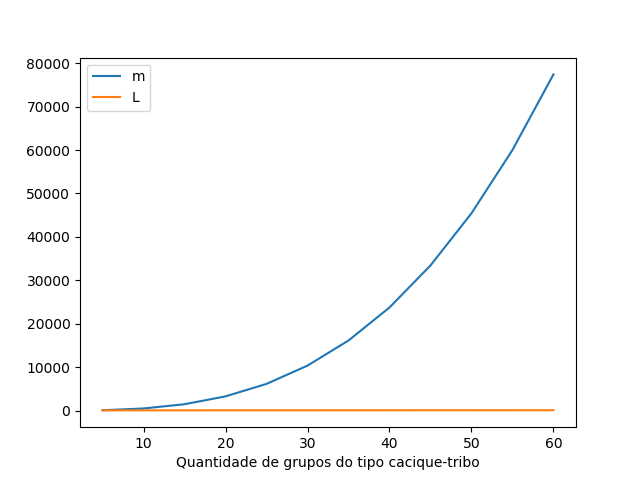
\includegraphics[width=0.7\linewidth]{figure_m_L.png}
  				\caption{Comparação dos valores de m e L} \label{fig:M1}
			\end{figure}

			É visível que o valor de $L$ aumenta muito menos em comparação com o aumento de m. Logo o impacto de L é baixo, então podemos considerar a complexidade do algoritmo como sendo $O(n^2)$.

			Possíveis testes que poderiam ser feitos seria aumentar o número de grupos de \emph{cacique-tribo} e checar se $L$ começa a tender a algum valor conforme maior fica o valor de $m$ ou até mesmo provar de alguma forma álgebrica, se exisitir.
			\begin{figure}[h]
  				\centering
  				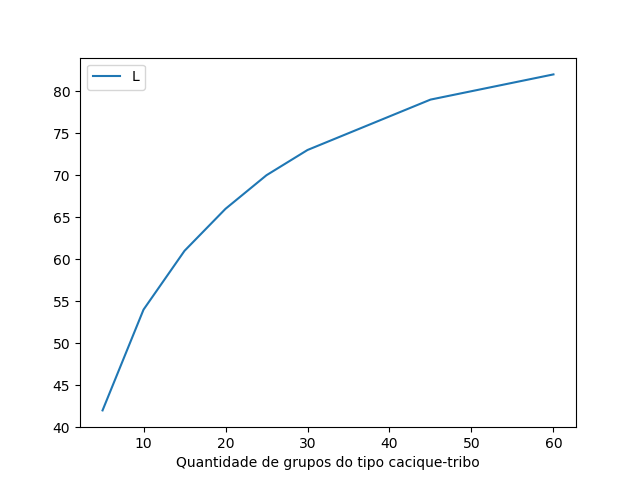
\includegraphics[width=0.7\linewidth]{figure_L.png}
  				\caption{Aumento dos valores de L conforme o aumento dos grupos} \label{fig:M1}
			\end{figure}


	\subsection{Comparação entre os métodos}
		
		O fato do método Interativo possuir complexidade $O(n^2)$ e o método de escalonamento por Eliminação Gaussiana, $O(n^3)$, o torna extremamente mais eficiente. No gráfico abaixo percebemos a diferença significativa entre os dois algoritmos. Mais testes acabaram por ser uma limitação, já que depois de 60 grupos, os testes começaram a demorar mais 7 minutos utilizando o método de escalonamento, mesmo não demorando nem 2 segundos utilizando o método interativo.
		
		\begin{figure}
  			\centering
  			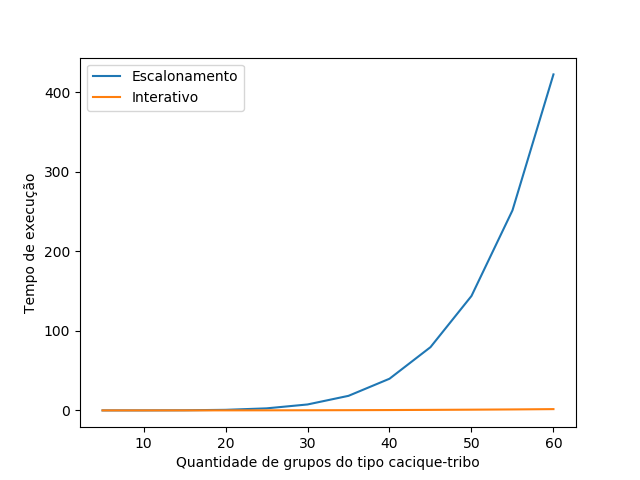
\includegraphics[width=0.7\linewidth]{comparacao_e_i.png}
  			\caption{Comparação do tempo de execução de cada método em grafos do tipo cacique-tribo}  \label{fig:M1}
		\end{figure}
		
		\begin{figure}
  			\centering
  			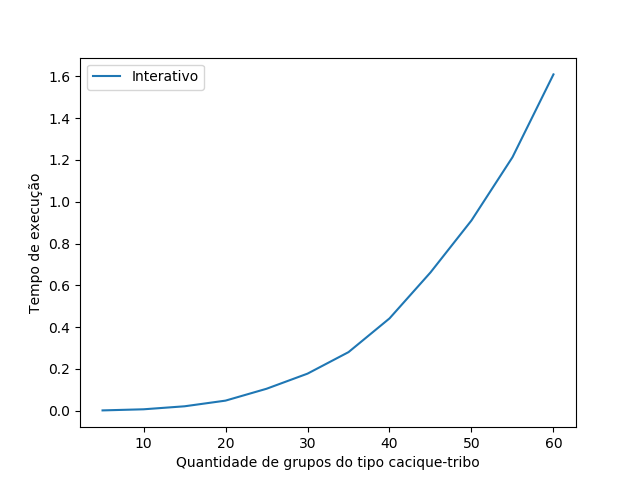
\includegraphics[width=0.7\linewidth]{interativo.png}
  			\caption{Tempo de execução do método Interativo} \label{fig:M1}
		\end{figure}
		
\newpage

\vspace{3em}

\section{Programa}
	O programa foi feito em Python (3.7), com uso da biblioteca \emph{time}, afim de calcular o tempo de execução de cada método. A entrada do programa consiste na entrada do grafo respectivo a rede de páginas que deve ser analisada. Para leitura do grafo foi usado uma forma de representação chamada Lista de Adjacências que consiste em criar um vetor para cada vértice do grafo, esse vetor tem todos os vértices para o qual o vértice aponta (tem uma aresta). A utilização desse método de representação foi feita de modo possibilitar uma maior facilidade na visualização do que está sendo inserido.
		
	Usando o grafo da Figura 1 como exemplo, a entrada do exemplo no programa fica a seguinte:
	
		\begin{lstlisting}
			5 			 	# Numeros de grafos
			0.15 		# Alpha
			1 2				# Vertice u aponta para o Vertice v
			1 4
			2 1
			3 4
			3 5
			4 2
			5 1
			0 0				# Fim da insercao de arestas
													(Um dos valores igual a 0)
		\end{lstlisting}
	
	A saída consiste em opções de classificação do rank de acordo com cada método (Digite L ou S), que também permite informar quantos primeiros do rank você deseja ver, e análise dos métodos (Digite A), que mostra tempo de execução de cada método, número de repetições do método interativo, maior e menor diferença entre as importâncias calculada por cada método, etc. Também foram feitos testes automatizados usando Shell script e o progrma em Python alterado para salvar os resultados como arquivo texto, e alguns dos seus resultados foram vistos nas seções anteriores. Esses testes, seus resultados e o arquivo do progama alterado podem ser encontrados no Github\footnote{https://github.com/pedro913/pageRank}, que também contém resultados de outros testes.
	
\vspace{3em}

\section{Tarefas}
	Na seção serão visto os resultados dos testes proposto a serem feitos. Além disso, como a entrada do grafo é feita através de uma Lista de Adjacências, foi montado um programa em Python a fim de criar arquivos de texto com as entradas do grafo para Tarefa 2 (podendo ser encontrado na página do Github mencionada anteriormente). É importante levar em conta que os resultados foram feitos com um processador Ryzen 5 2400G que é um pouco melhor do que a média de processadores que as pessoas costumam ter, afetando diretamente o tempo de execução do programa. Os resultados dos testes são mostrados a seguir.
	
	\subsection{Tarefa 1}
		Está tarefa consistia na criação do programa computacional que gerasse o ranking de importância das páginas. Também foi proposto um primeiro teste que consiste na seguinte rede de páginas:
		
		\begin{figure}[h]
  			\centering
  			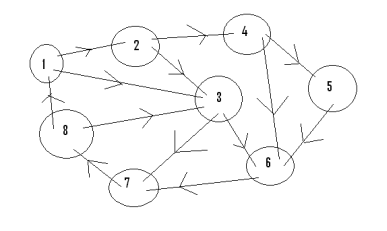
\includegraphics[width=0.45\linewidth]{t_1_exemplo.png}
  			\caption{Tarefa 1} \label{fig:M1}
		\end{figure}	 
		Segue uma análise do teste:\\
		
		\begin{lstlisting}
			Tempo de execucao:
		 			Escalonamento: 	 0.00017 segundos
		 			Interativo: 	 	 	0.00057 segundos 

			Numero de repeticoes metodo interativo: 47 

			Diferenca: 
		 			Maior: 	 7.066221e-08
		 			Menor: 	 8.008726e-10 

			Rank: 
		 		Pagina mais importante e menos importante:
		 	 		Escalonamento: 	 7 e 5
		 	 		Interativo: 	 	 	7 e 5
		\end{lstlisting}
		
	\subsection{Tarefa 2}
		Nessa tarefa 2 foi feito várias análises das redes do tipo \emph{cacique-tribo} construídas de uma forma padronizada, algumas foram já mostradas como gráficos mostrando o aumento do $m$ em relação ao aumento de $L$ entre 5 a 60 grupos. Como dito no começo da seção, também foi feito um programa para criação de teste para essa rede, assim possibilitando a construção de gráficos de forma mais fácil. Também com análise dos teste é perceptível que as páginas com o maior número de ligações tendem a se beneficiar mais dessas redes, mostrando que o cacique com o maior número de páginas ligada a ele é a página com maior importância:\\
		
		\lstset{xrightmargin=150pt,}
		
		\begin{lstlisting}
			Grupos			Pagina mais importante
					10												55
					20												210
					30												465
					40												820
					50												1275
					60												1830
			
		\end{lstlisting}
		Perceba que em todos os casos a página mais importante é aquela que é cacique do grupo com maior número de índios. Também foi visto, através de testes, que a página com menor importância sempre será a página 2.
		
		Análise dos resultados gerados pelo programa para uma rede \emph{cacique-tribo} com 20 grupos gerados da forma descrita na relatório de apresentação do projeto:\\
			
		\lstset{xrightmargin=70pt,}
		\begin{lstlisting}
			Tempo de execucao:
		 			Escalonamento: 	 0.71597 segundos
		 			Interativo: 	 	 	0.05024 segundos 

			Numero de repeticoes metodo interativo: 66 

			Diferenca: 
		 			Maior: 	 6.222227e-10
		 			Menor: 	 6.692177e-12

			Rank: 
		 		Pagina mais importante e menos importante:
		 	 		Escalonamento: 	 210 e 2
		 	 		Interativo: 	 	 	210 e 2
		\end{lstlisting}
		
		Análise dos resultados gerados pelo programa para uma rede \emph{cacique-tribo} com 40 grupos gerados da forma descrita na relatório de apresentação do projeto:\\
		
		\begin{lstlisting}
			Tempo de execucao:
		 			Escalonamento: 	 39.82074 segundos
		 			Interativo: 	 	 	 0.44823 segundos

			Numero de repeticoes metodo interativo: 77 

			Diferenca: 
		 			Maior: 	 3.890358e-11
		 			Menor: 	 3.286249e-13

			Rank: 
		 		Pagina mais importante e menos importante:
		 	 		Escalonamento: 	 820 e 2
		 	 		Interativo: 	 	 	820 e 2
		\end{lstlisting}
		
		Devido ao processador, os testes podem ser considerados lentos, considerando que existem super-computadores para fazer esses cálculos que processam uma quantidade muito maior de dados em um tempo muito menor, ou rápido, se comparado com testes feito por outros computadores com processadores não tão modernos. Fora isso, é evidente a melhora em tempo de execução quando utilizamos o método Interativo ao invés do método por Escalonamento. No teste com 40 grupos, o algoritmo Interativo é aproximadamente 88 vezes mais rápido que o por Escalonamento. Já com 60 grupos, 262 vezes mais rápido.
\end{document}
